\section{The Primadona-Monatip through-trip: impressions}

\margininbox{Primadona-Monatip}{
     \begin{itemize}
    \item Miriam Ridao
    \item Iztok Mo\v{z}ir
    \item Dan Greenwald
    \item Sam Page
    \item Isha Kaur
    \item William French
    \end{itemize}}{\explo}


Izi and Zdenko had both come up the mountain, and as they knew the \passage{Primadona}/\passage{Monatip} system better than anyone they offered to take some of us to see parts of the cave we hadn't gone to. Two teams were formed: Izi's `lazy' team, consisting of Izi, Isha, Sam, Dan, Will F and myself, and Zdenko's team for those who wanted more of a challenge, who were Zdenko, Rhys and Will S. Zdenko and Co. left early in the morning, but we opted for a more relaxed approach and didn't leave until midday. Our plan was to reach \passage{Alkatraz} in \passage{Monatip}, and to spend some time looking around the chamber for the passage previously discovered by Tetley (but never recorded) that would lead to \passage{Primadona}, creating a new connection between the two caves.

Morale was high as we set off for the caves, and as it was still early days the abseil to the entrance series was still new and exciting, and not at all soul-destroying. I had gone to the cave only twice before and had never gone deeper than around 200\,m, so I was excited to see more.


We moved swiftly through the entrance series, descending pitch after pitch until we met Jack and Kenneth near \passage{Bear Pitch}. They were busy rebolting a pitch head, and unfortunately this meant we had to start using the old rope. This was my first taste of Slovenian style caving, and although I can appreciate the economical approach to bolts and rope, I'm not sure how safe it was. We carried on, and at \passage{Risanke} (RIP\sidenote{See Arun's rescue, in which explosives were used to widen this previously entertaining passage.}) we passed Zdenko, Rhys and Will S. They had gone to \passage{Smer0} and were on their way out. Izi had forgotten to write a call out in the log book, so this was a good opportunity to send a message up to the surface. We soon reached \passage{Lost and Found}, a junction where the cave passage deviated -- one path lead deeper into \passage{Primadona} and to \passage{Quantum State}, but the path we were interested in would take us into \passage{Monatip}. 

Progress became much slower and we would occasionally have to stop and look for possible ways on as it had been a while since Izi had done the connection and he was struggling to remember certain parts. Our longest stop happened at an aven where the way on turned out to be a hidden free-climb up a waterfall\sidenote{where later Grega Maffi and Tanguy Racine would be halted on their attempt at the through-trip}.

After a while, we reached \passage{Alkatraz}, where we stopped and half-heartedly looked around for a while. Although this had been our purpose in coming, we were all tired from the journey and eager to move on. It was here that we decided to carry on and exit through the \passage{Monatip} entrance, rather than retrace our steps back through \passage{Primadona}. 

\begin{figure*}[t!]
\checkoddpage \ifoddpage \forcerectofloat \else \forceversofloat \fi
\centering
\frame{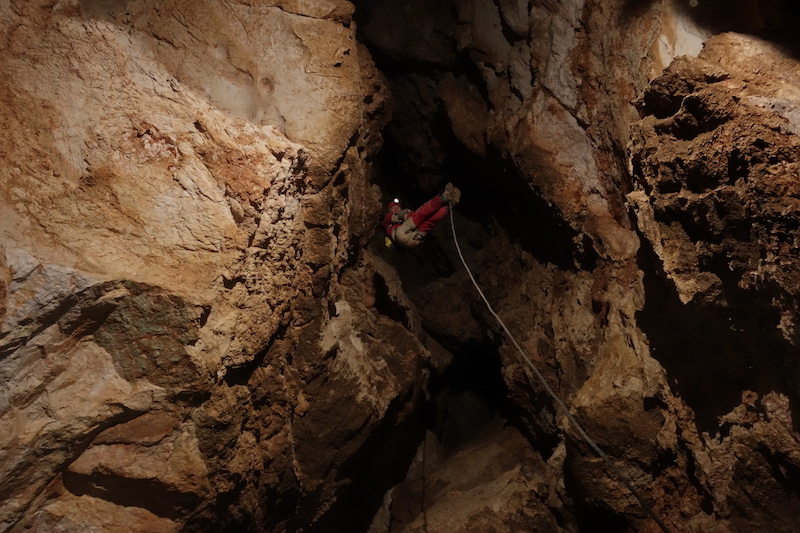
\includegraphics[width=\textwidth]{images/2016/miriam-2016/zdenko-2016.jpg}}
\caption[][-15pt]{Zdenko, a senior JSPDT caver descending the pitch dubbed `\protect\passage{Knot Very Good}', which drops into \protect\passage{Galerija} \pic{Rhys Tyers}}
\label{Zdenko16}
\end{figure*}
From that point on the caving became less SRT based and more technically demanding, and although this was more tiring, I was glad for the break. \bignote{After lots of flat out crawling - during which I was bombarded with flashbacks of the T shaped passage in \passage[the best cave]{King Pot}}- and many free climbs later, we eventually reached a very tight squeeze that opened out into a slightly larger chamber. To get through the crack I had to take off my SRT bag for the first time. This made the squeeze slightly easier but no less terrifying. Everyone slowly made their way through, and on the whole it was only mildly traumatic.

After going through a series of unpleasant crawls, we realised that we wouldn't make it out in time for our call out, so Dan was sent ahead as we hoped he would move quicker on his own.

The rest of the cave was much easier, and although progress was still slow we eventually found the entrance to \passage{Monatip}, although as it was pitch black outside it took me a while to realise it wasn't another chamber, and actually the outside world. 

It was an exciting and challenging cave, and overall an amazing experience. 9/10
\name{Miriam Ridao}

\section{First findings: Quantum State and below Terminus}
\margininbox{Quantum State}{
\begin{citemize}
\item Miriam Ridao 
\item Kenneth Tan
\item Rhys Tyers
\item William French
\end{citemize}}{\explo}
After discovering \passage{Quantum State} with Rhys and Kenneth and leaving the lead unpushed, a few days later I went back down with Will French. 

Uncertain of how much passage we would find, we brought only a small hand bolting kit with us instead of the heavy drills, and rather than bringing a tackle sack full of rope we planned to pick one up on the way down. 

We went through the abseil and down the entrance series without any problems, although \passage{Risanke} (RIP) was where we started to lose our way a bit. Will had not gone down this far, so it was up to me to lead the way to \passage{Quantum State}. We eventually reached the \passage{Quantum State} entrance pitch, although it hadn't been a smooth journey - I often forgot the way on, and during one descent my hair got caught in my descender. It was the first time I'd brought the super friends down into the caves with me, so I could cut the jammed hair off with minimal trauma, but from then on I made sure to keep my hair well away from the rope.

\margininbox{The Rap}{
In Primadona with Kenneth and Miriam,\\
Going caving in search of a million\\
metres of passage,\\
spreading the message,\\
there's unexplored crevice.\\
\protect\mininame{Rhys Tyers}
}{\logbook}

We descended down the \passage{Quantum State} entrance pitch and quickly reached the PSS survey station marking the edge of discovered passage. After a few short metres we found an intersection, where the passage split into two paths. The more unpleasant looking passage followed a stream, and after pursuing it for a bit as the ceiling got lower and the walls got narrower, we found a sump. Reluctant to survey, we turned back, hoping that the other path would reveal more. 

A short, awkward crawl later and we reached a pitch. Excited that the lead wasn't dead, we quickly(ish) hand bolted the pitch head - my first experience of hand bolting. After adding the hanger, we realised that we had left the spanner back at the \passage{Bivi}. Will was keen to go down and said he didn't mind descending on a single bolt with a semi screwed on hanger, but I had had enough of Slovenian style rigging, so instead we went back up and decided to come back another time.

The next day, armed with a spanner, we completed the bolting, and after some struggling with the rigging (I'd only rigged once before), we descended down, destroying the previously pristine mud floor in the process. 

Almost immediately it was clear that there was no obvious way on, although \bignote{after some desperate searching, we found a small crack in the wall} above a short free climb. Will went through first, and tried in vain to hammer away at the edges, after which I followed through. The chamber on the other side was beautifully untouched, with a small waterfall (a trickle of water) creating a small pool at our feet. There were, again, no obvious leads, but deciding that we had gone through too much effort to turn back, we looked around carefully. After a dodgy free climb to reach the start of the waterfall I found a tight, dank passage following the stream. This, however, led to yet another sump, so we called it a day and started to survey back. 

Surveying proved to be especially unpleasant, as we were knee deep in water when surveying the sumps, but as we hadn't discovered much passage, it thankfully ended soon.
\name{Miriam Ridao}
